\documentclass{standalone}
\usepackage{tikz}
\usetikzlibrary{patterns, positioning}
\usepackage[sfdefault]{ClearSans} %% option 'sfdefault' activates Clear Sans as the default text font
\usepackage[T1]{fontenc}

\begin{document}
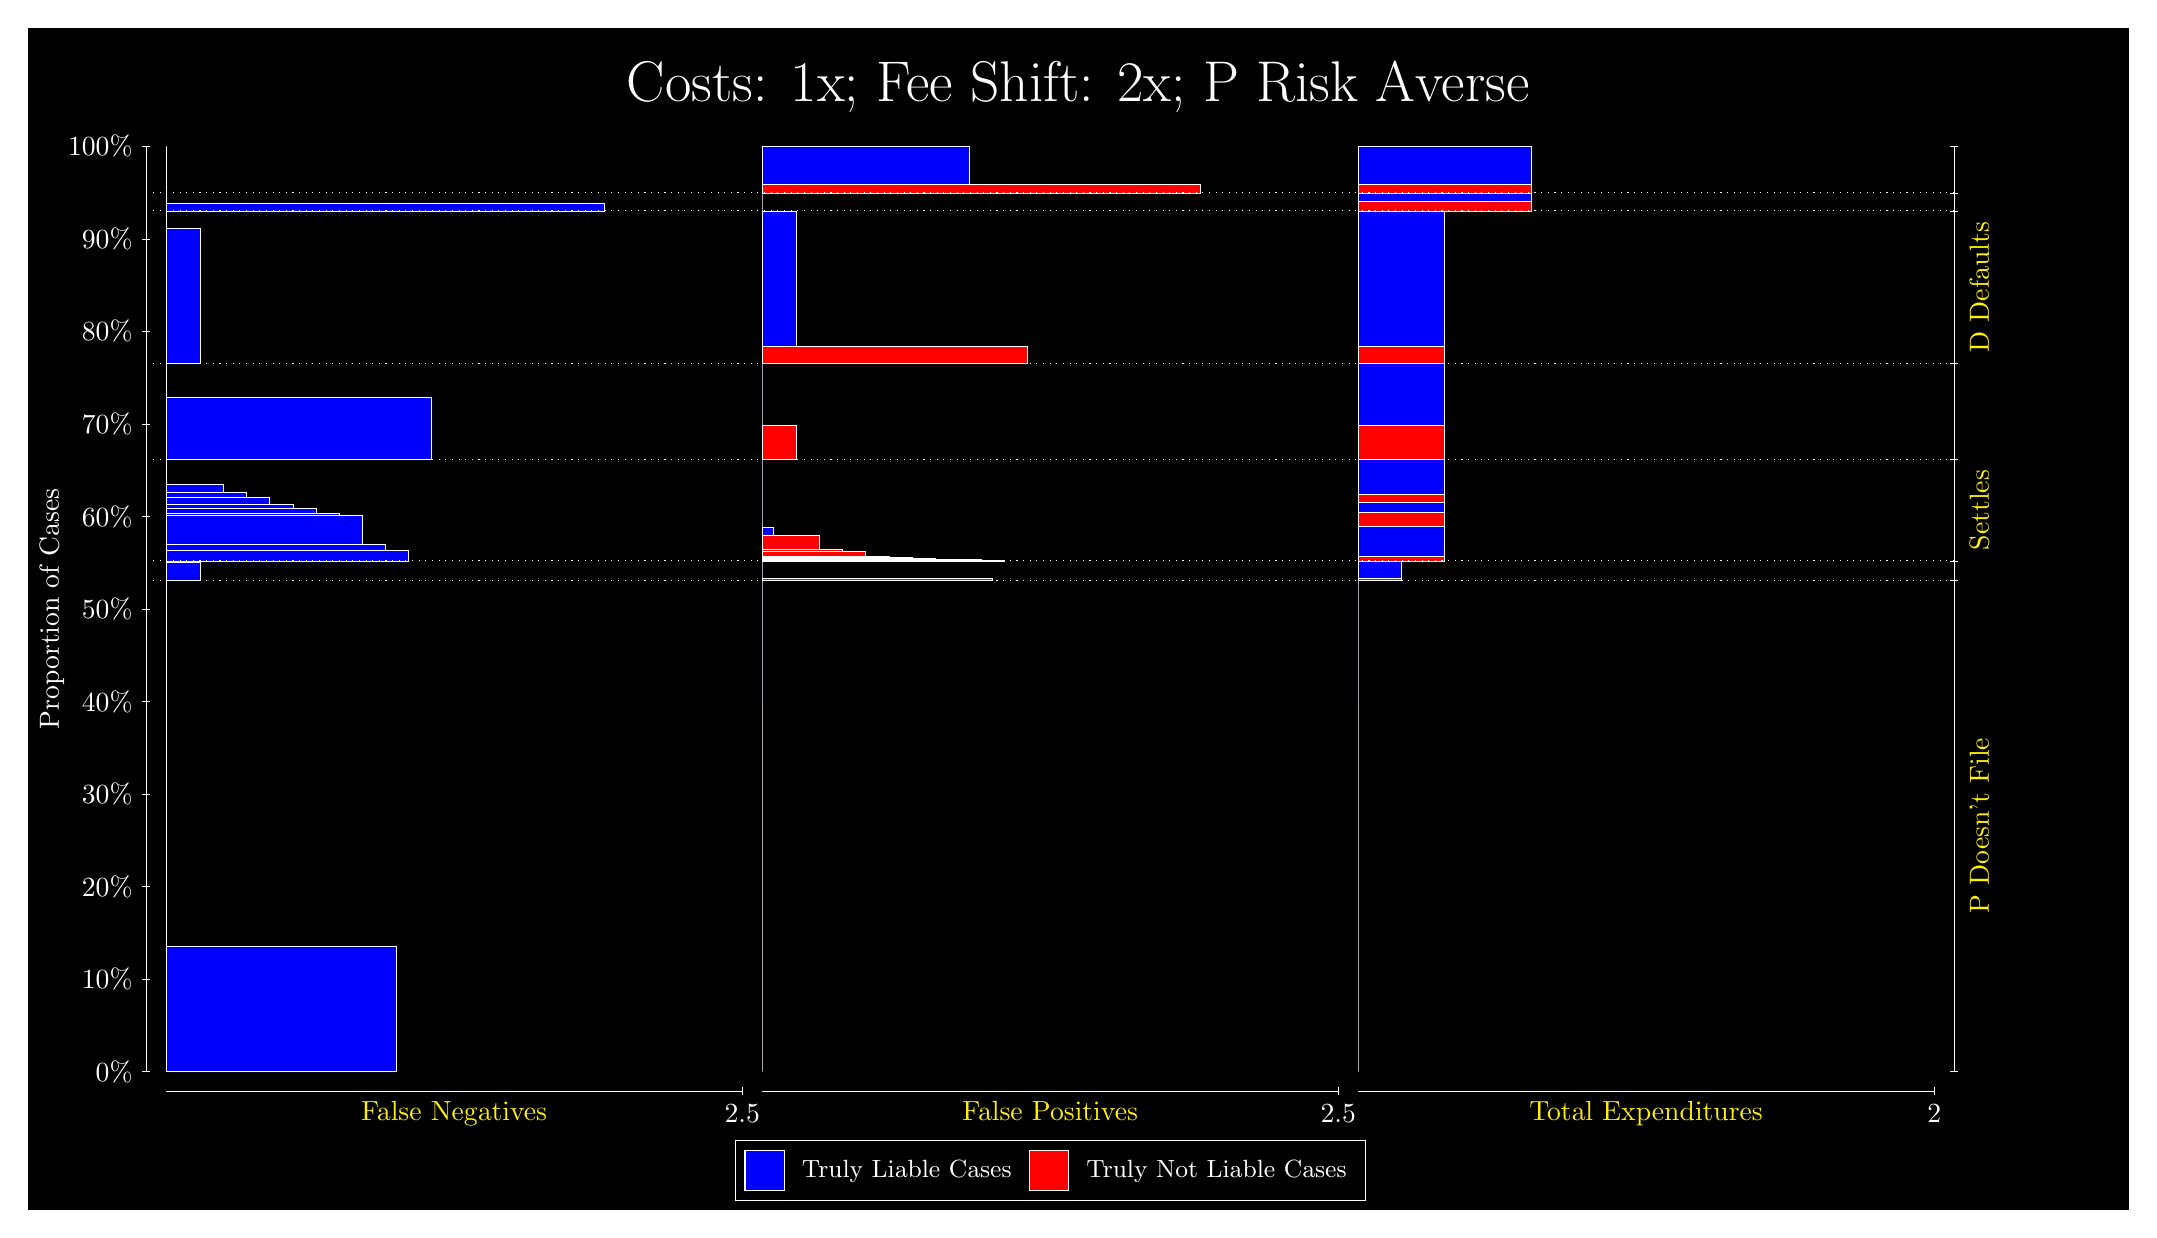
\begin{tikzpicture}
\draw[fill=black] (0,0) rectangle (26.667,15);
\draw[text=white] (0,13.5) rectangle (26.667,15) node[midway] {\huge Costs: 1x; Fee Shift: 2x; P Risk Averse};
\draw[white, very thin] (1.5,1.75) -- (1.5,13.5);
\node[rotate=90, text=white, anchor=center] at (0.3, 7.625) {Proportion of Cases};
\draw[white, very thin] (1.45,1.75) -- (1.55,1.75);
\node[text=white, anchor=east] at (1.45, 1.75) {0\%};
\draw[white, very thin] (1.45,2.925) -- (1.55,2.925);
\node[text=white, anchor=east] at (1.45, 2.925) {10\%};
\draw[white, very thin] (1.45,4.1) -- (1.55,4.1);
\node[text=white, anchor=east] at (1.45, 4.1) {20\%};
\draw[white, very thin] (1.45,5.275) -- (1.55,5.275);
\node[text=white, anchor=east] at (1.45, 5.275) {30\%};
\draw[white, very thin] (1.45,6.45) -- (1.55,6.45);
\node[text=white, anchor=east] at (1.45, 6.45) {40\%};
\draw[white, very thin] (1.45,7.625) -- (1.55,7.625);
\node[text=white, anchor=east] at (1.45, 7.625) {50\%};
\draw[white, very thin] (1.45,8.8) -- (1.55,8.8);
\node[text=white, anchor=east] at (1.45, 8.8) {60\%};
\draw[white, very thin] (1.45,9.975) -- (1.55,9.975);
\node[text=white, anchor=east] at (1.45, 9.975) {70\%};
\draw[white, very thin] (1.45,11.15) -- (1.55,11.15);
\node[text=white, anchor=east] at (1.45, 11.15) {80\%};
\draw[white, very thin] (1.45,12.325) -- (1.55,12.325);
\node[text=white, anchor=east] at (1.45, 12.325) {90\%};
\draw[white, very thin] (1.45,13.5) -- (1.55,13.5);
\node[text=white, anchor=east] at (1.45, 13.5) {100\%};

\draw[white, very thin] (24.457,1.75) -- (24.457,13.5);
\draw[white, very thin] (24.407,1.75) -- (24.507,1.75);
\node[anchor=west] at (24.407, 1.75) {};
\draw[white, very thin] (24.407,7.9902) -- (24.507,7.9902);
\node[anchor=west] at (24.407, 7.9902) {};
\draw[white, very thin] (24.407,8.2349) -- (24.507,8.2349);
\node[anchor=west] at (24.407, 8.2349) {};
\draw[white, very thin] (24.407,9.5269) -- (24.507,9.5269);
\node[anchor=west] at (24.407, 9.5269) {};
\draw[white, very thin] (24.407,10.742) -- (24.507,10.742);
\node[anchor=west] at (24.407, 10.742) {};
\draw[white, very thin] (24.407,12.68) -- (24.507,12.68);
\node[anchor=west] at (24.407, 12.68) {};
\draw[white, very thin] (24.407,12.909) -- (24.507,12.909);
\node[anchor=west] at (24.407, 12.909) {};
\draw[white, very thin] (24.407,13.5) -- (24.507,13.5);
\node[anchor=west] at (24.407, 13.5) {};

\draw[white, very thin, fill=blue] (1.75,1.75) rectangle (4.6775,3.335);
\draw[white, very thin, fill=red] (1.75,3.335) rectangle (1.75,7.9902);
\draw[white, very thin, fill=blue] (1.75,7.9902) rectangle (2.1891,8.2142);
\draw[white, very thin, fill=red] (1.75,8.2142) rectangle (1.75,8.2349);
\draw[white, very thin, fill=blue] (1.75,8.2349) rectangle (4.8239,8.3705);
\draw[white, very thin, fill=blue] (1.75,8.3705) rectangle (4.5312,8.4479);
\draw[white, very thin, fill=blue] (1.75,8.4479) rectangle (4.2384,8.8093);
\draw[white, very thin, fill=blue] (1.75,8.8093) rectangle (3.9457,8.8455);
\draw[white, very thin, fill=blue] (1.75,8.8455) rectangle (3.6529,8.9084);
\draw[white, very thin, fill=blue] (1.75,8.9084) rectangle (3.3602,8.9589);
\draw[white, very thin, fill=blue] (1.75,8.9589) rectangle (3.0674,9.0369);
\draw[white, very thin, fill=blue] (1.75,9.0369) rectangle (2.7746,9.1036);
\draw[white, very thin, fill=blue] (1.75,9.1036) rectangle (2.4819,9.2053);
\draw[white, very thin, fill=red] (1.75,9.2053) rectangle (1.75,9.5269);
\draw[white, very thin, fill=blue] (1.75,9.5269) rectangle (5.1167,10.316);
\draw[white, very thin, fill=red] (1.75,10.316) rectangle (1.75,10.742);
\draw[white, very thin, fill=blue] (1.75,10.742) rectangle (2.1891,12.46);
\draw[white, very thin, fill=red] (1.75,12.46) rectangle (1.75,12.68);
\draw[white, very thin, fill=blue] (1.75,12.68) rectangle (7.3123,12.782);
\draw[white, very thin, fill=red] (1.75,12.782) rectangle (1.75,12.909);
\draw[white, very thin, fill=red] (1.75,12.909) rectangle (1.75,13.012);
\draw[white, very thin, fill=blue] (1.75,13.012) rectangle (1.75,13.5);
\draw[white, very thin, fill=red] (9.3189,1.75) rectangle (9.3189,6.4052);
\draw[white, very thin, fill=blue] (9.3189,6.4052) rectangle (9.3189,7.9902);
\draw[white, very thin, fill=red] (9.3189,7.9902) rectangle (12.246,8.0109);
\draw[white, very thin, fill=blue] (9.3189,8.0109) rectangle (9.3189,8.2349);
\draw[white, very thin, fill=red] (9.3189,8.2349) rectangle (12.393,8.2452);
\draw[white, very thin, fill=red] (9.3189,8.2452) rectangle (12.1,8.2525);
\draw[white, very thin, fill=red] (9.3189,8.2525) rectangle (11.807,8.2618);
\draw[white, very thin, fill=red] (9.3189,8.2618) rectangle (11.515,8.2703);
\draw[white, very thin, fill=red] (9.3189,8.2703) rectangle (11.222,8.2825);
\draw[white, very thin, fill=red] (9.3189,8.2825) rectangle (10.929,8.2874);
\draw[white, very thin, fill=red] (9.3189,8.2874) rectangle (10.929,8.2909);
\draw[white, very thin, fill=red] (9.3189,8.2909) rectangle (10.636,8.355);
\draw[white, very thin, fill=red] (9.3189,8.355) rectangle (10.344,8.379);
\draw[white, very thin, fill=red] (9.3189,8.379) rectangle (10.051,8.5565);
\draw[white, very thin, fill=blue] (9.3189,8.5565) rectangle (9.4652,8.6582);
\draw[white, very thin, fill=blue] (9.3189,8.6582) rectangle (9.3189,9.5269);
\draw[white, very thin, fill=red] (9.3189,9.5269) rectangle (9.758,9.9536);
\draw[white, very thin, fill=blue] (9.3189,9.9536) rectangle (9.3189,10.742);
\draw[white, very thin, fill=red] (9.3189,10.742) rectangle (12.686,10.963);
\draw[white, very thin, fill=blue] (9.3189,10.963) rectangle (9.758,12.68);
\draw[white, very thin, fill=red] (9.3189,12.68) rectangle (9.3189,12.808);
\draw[white, very thin, fill=blue] (9.3189,12.808) rectangle (9.3189,12.909);
\draw[white, very thin, fill=red] (9.3189,12.909) rectangle (14.881,13.012);
\draw[white, very thin, fill=blue] (9.3189,13.012) rectangle (11.954,13.5);
\draw[white, very thin, fill=red] (16.888,1.75) rectangle (16.888,6.4052);
\draw[white, very thin, fill=blue] (16.888,6.4052) rectangle (16.888,7.9902);
\draw[white, very thin, fill=red] (16.888,7.9902) rectangle (17.437,8.0109);
\draw[white, very thin, fill=blue] (16.888,8.0109) rectangle (17.437,8.2349);
\draw[white, very thin, fill=red] (16.888,8.2349) rectangle (17.986,8.2874);
\draw[white, very thin, fill=blue] (16.888,8.2874) rectangle (17.986,8.6726);
\draw[white, very thin, fill=red] (16.888,8.6726) rectangle (17.986,8.8501);
\draw[white, very thin, fill=blue] (16.888,8.8501) rectangle (17.986,8.9857);
\draw[white, very thin, fill=red] (16.888,8.9857) rectangle (17.986,9.0773);
\draw[white, very thin, fill=blue] (16.888,9.0773) rectangle (17.986,9.5269);
\draw[white, very thin, fill=red] (16.888,9.5269) rectangle (17.986,9.9536);
\draw[white, very thin, fill=blue] (16.888,9.9536) rectangle (17.986,10.742);
\draw[white, very thin, fill=red] (16.888,10.742) rectangle (17.986,10.963);
\draw[white, very thin, fill=blue] (16.888,10.963) rectangle (17.986,12.68);
\draw[white, very thin, fill=red] (16.888,12.68) rectangle (19.083,12.808);
\draw[white, very thin, fill=blue] (16.888,12.808) rectangle (19.083,12.909);
\draw[white, very thin, fill=red] (16.888,12.909) rectangle (19.083,13.012);
\draw[white, very thin, fill=blue] (16.888,13.012) rectangle (19.083,13.5);
\draw[white, dotted] (1.5,7.9902) -- (24.457,7.9902);
\draw[white, dotted] (1.5,8.2349) -- (24.457,8.2349);
\draw[white, dotted] (1.5,9.5269) -- (24.457,9.5269);
\draw[white, dotted] (1.5,10.742) -- (24.457,10.742);
\draw[white, dotted] (1.5,12.68) -- (24.457,12.68);
\draw[white, dotted] (1.5,12.909) -- (24.457,12.909);
\draw[white, very thin] (1.75,1.5) -- (9.0689,1.5);
\node[text=yellow, anchor=north] at (5.4094, 1.5) {False Negatives};
\draw[white, very thin] (9.0689,1.45) -- (9.0689,1.55);
\node[text=white, anchor=north] at (9.0689, 1.45) {2.5};

\draw[white, very thin] (9.3189,1.5) -- (16.638,1.5);
\node[text=yellow, anchor=north] at (12.978, 1.5) {False Positives};
\draw[white, very thin] (16.638,1.45) -- (16.638,1.55);
\node[text=white, anchor=north] at (16.638, 1.45) {2.5};

\draw[white, very thin] (16.888,1.5) -- (24.207,1.5);
\node[text=yellow, anchor=north] at (20.547, 1.5) {Total Expenditures};
\draw[white, very thin] (24.207,1.45) -- (24.207,1.55);
\node[text=white, anchor=north] at (24.207, 1.45) {2};

\node[text=yellow, centered, rotate=90] at (24.777, 4.8701) {P Doesn't File};

\node[text=yellow, centered, rotate=90] at (24.777, 8.8809) {Settles};

\node[text=yellow, centered, rotate=90] at (24.777, 11.711) {D Defaults};



\draw (12.978300999999998,1.5) node[draw=none] (baseCoordinate) {};
\begin{scope}[align=center]
        \matrix[scale=0.5, draw=white, below=0.5cm of baseCoordinate, nodes={draw}, column sep=0.1cm]{
            \node[rectangle, draw, minimum width=0.5cm, minimum height=0.5cm, fill=blue] {}; &
            \node[draw=none, font=\small, text=white] (B) {Truly Liable Cases}; &
            \node[rectangle, draw, minimum width=0.5cm, minimum height=0.5cm, fill=red] {}; &
            \node[draw=none, font=\small, text=white] (B) {Truly Not Liable Cases}; \\
            };
\end{scope}

\end{tikzpicture}
\end{document}